% !TeX root = ../\dfrac{numeratore}{denominatore}report.tex

\part{Design}


bla bla bla

\chapter{Main Actors}
The application has three main actors:
\begin{itemize}
	\item Client
	\item TIMS
	\item Statician
\end{itemize}

\paragraph{Client}
this user is able to view map and run searches on it and he’s also able to ask 
for directions between two points on the map. The user don't need to be registered to use the application. With correct use of the app, the client can avoid inconvenience during their journey in the city of London, completing his visit in safety and minimizing delays.

\paragraph{TIMS}
this user is able to perform CRUD operations on the disruptions. TIMS, in pratics, is an API provided by Transport For London.

\paragraph{Statician}
this user is able to perform analytics on the data generated by TIMS. The statician can access his panel inserting the correct username and password. By acceding this panel he can view some different graphs that are useful to make statistics about security when travelling in London. Using these results, the statistician can identify critical issues in the city of London and suggest to the authorities any changes to traffic or simply indicate which areas are the most critical from this point of view.

\chapter{Functional requirements}

The application will allow its users to perform the following tasks:

\section{Client}

\begin{itemize}
	\item \textbf{View the map}
	\item \textbf{Move the map in a direction}, with the typical drag 'n drop
	\item \textbf{Increase or decrease the map magnifying}, with either buttons 
	or the mouse's wheel
	\item \textbf{Search for a specific place}, the following method are 
	supported:
	\begin{itemize}
		\item With an address
		\item With a POI's name
		\item With WGS84 geographical coordinates
	\end{itemize}
	\item \textbf{Ask for directions} between two intersections on the map
	\begin{itemize}
		\item Via car
		\item Via bicycle
		\item On foot
	\end{itemize}
	\item \textbf{Calculate the estimate time of travel}
	\item \textbf{View the path} on the map
	\item \textbf{View active disruptions' and POIs' informations}
	\item \textbf{View a suggestion list of POIs}, based on the string the user insert in the appropriate area
	\item \textbf{Refresh active disruptions' data} clicking on the refresh button
	\item \textbf{Choose if to consider or not disruptions} during the route calculation 
\end{itemize}
\section{TIMS}
	\begin{itemize}
	\item \textbf{Create/Update a disruption}
	\item \textbf{Close a disruption}
	\end{itemize}
\section{Statician}
\begin{itemize}
	\item \textbf{Access the analytics tools}
	\item \textbf{Display the disruptions' heatmap}, chosen a certaine class
	\item \textbf{Choose the precision of the hehatmap between three grades:}
		\begin{itemize}
		\item High
		\item Medium
		\item Low
		\end{itemize}
	\item \textbf{Visualize a graph about hourly statistics chosen a class of disruption}
	\item \textbf{Visualize a table that contains the most common disruption for each severity considering the area actually displayed on the screen}
	\item \textbf{Update the table}
\end{itemize}
\chapter{Not functional requirements}
	\begin{itemize}
	\item To solve a routing problem in an acceptable amount of time
	\item A cache for queries to have a better response time for frequent queries
	\item To find a good approximation of the optimal route
	\item Respect the access constraints on the graph, such as oneway streets
	\item Use a routing algorithm that uses an heuristic function to compute a path, such as A*, to avoid excessive exploration of the hypothesis space, since those algorithms are always exponential in the graph’s dimension
	\item Define a good heuristic to guide the algorithm on its visit on the graph, considering features such as the road’s classification, speed limit, the geographical distance between the vertices.
	\end{itemize}
\chapter{CAP Theorem issue}

In order to optimize performance for the anticipated high volume of read operations, it is essential to prioritize both high availability and low latency in the design of this application. Additionally, it is crucial that the system remains functional in the event of a partition.According to the CAP theorem, the design of this application should prioritize \textbf{Availability (A)} and \textbf{Partition Tolerance (P)} over Consistency (C). This means that the application is more focused on maintaining access to the system and tolerating partitioning rather than ensuring complete consistency of data.
\begin{figure}[H]
	\centering
	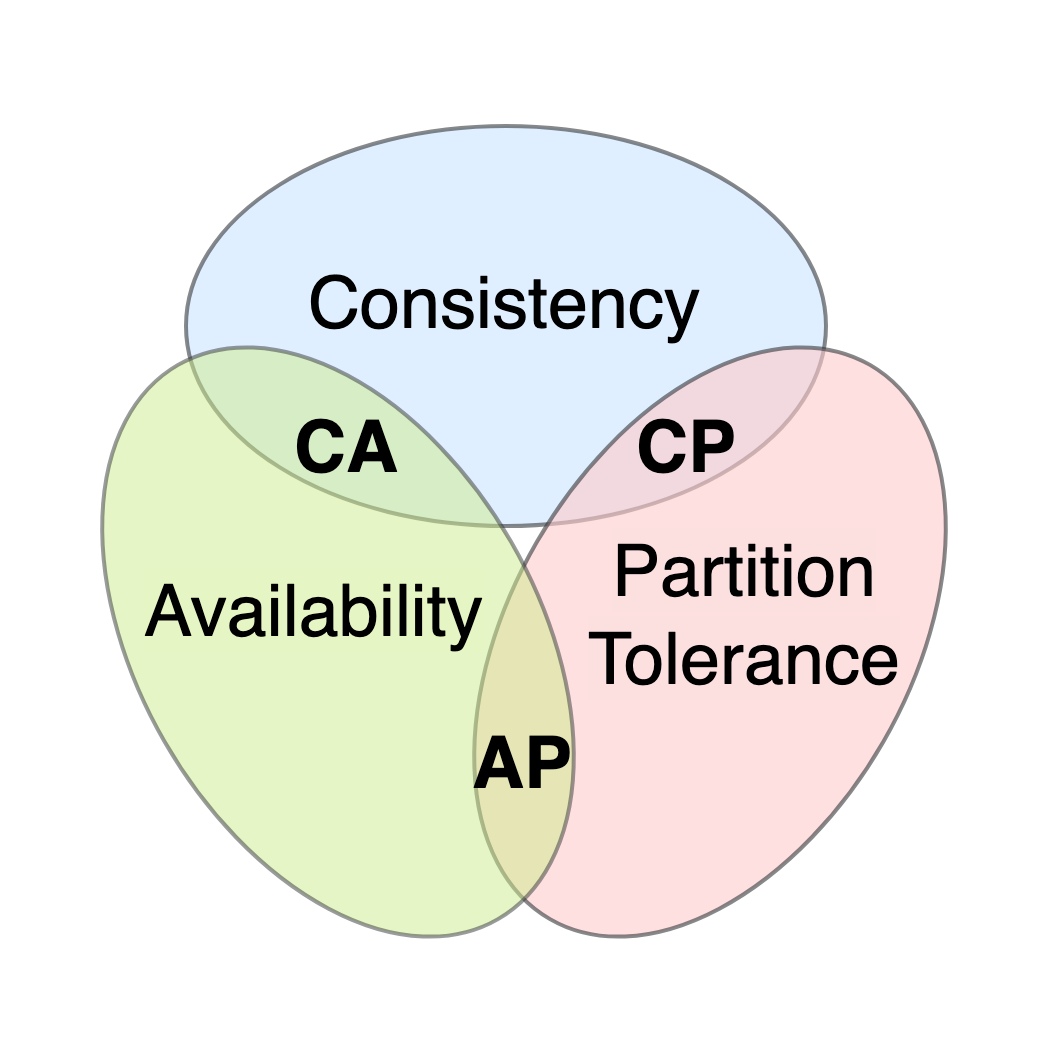
\includegraphics[width=0.4\linewidth]{assets/CAP_Theorem_Venn_Diagram}
	\caption{CAP theorem Venn diagram}
	\label{fig:captheoremvenndiagram}
\end{figure}
\chapter{Use cases}

\chapter{Databases design}

%TODO INCLUDE PDF WHEN COMPILING
%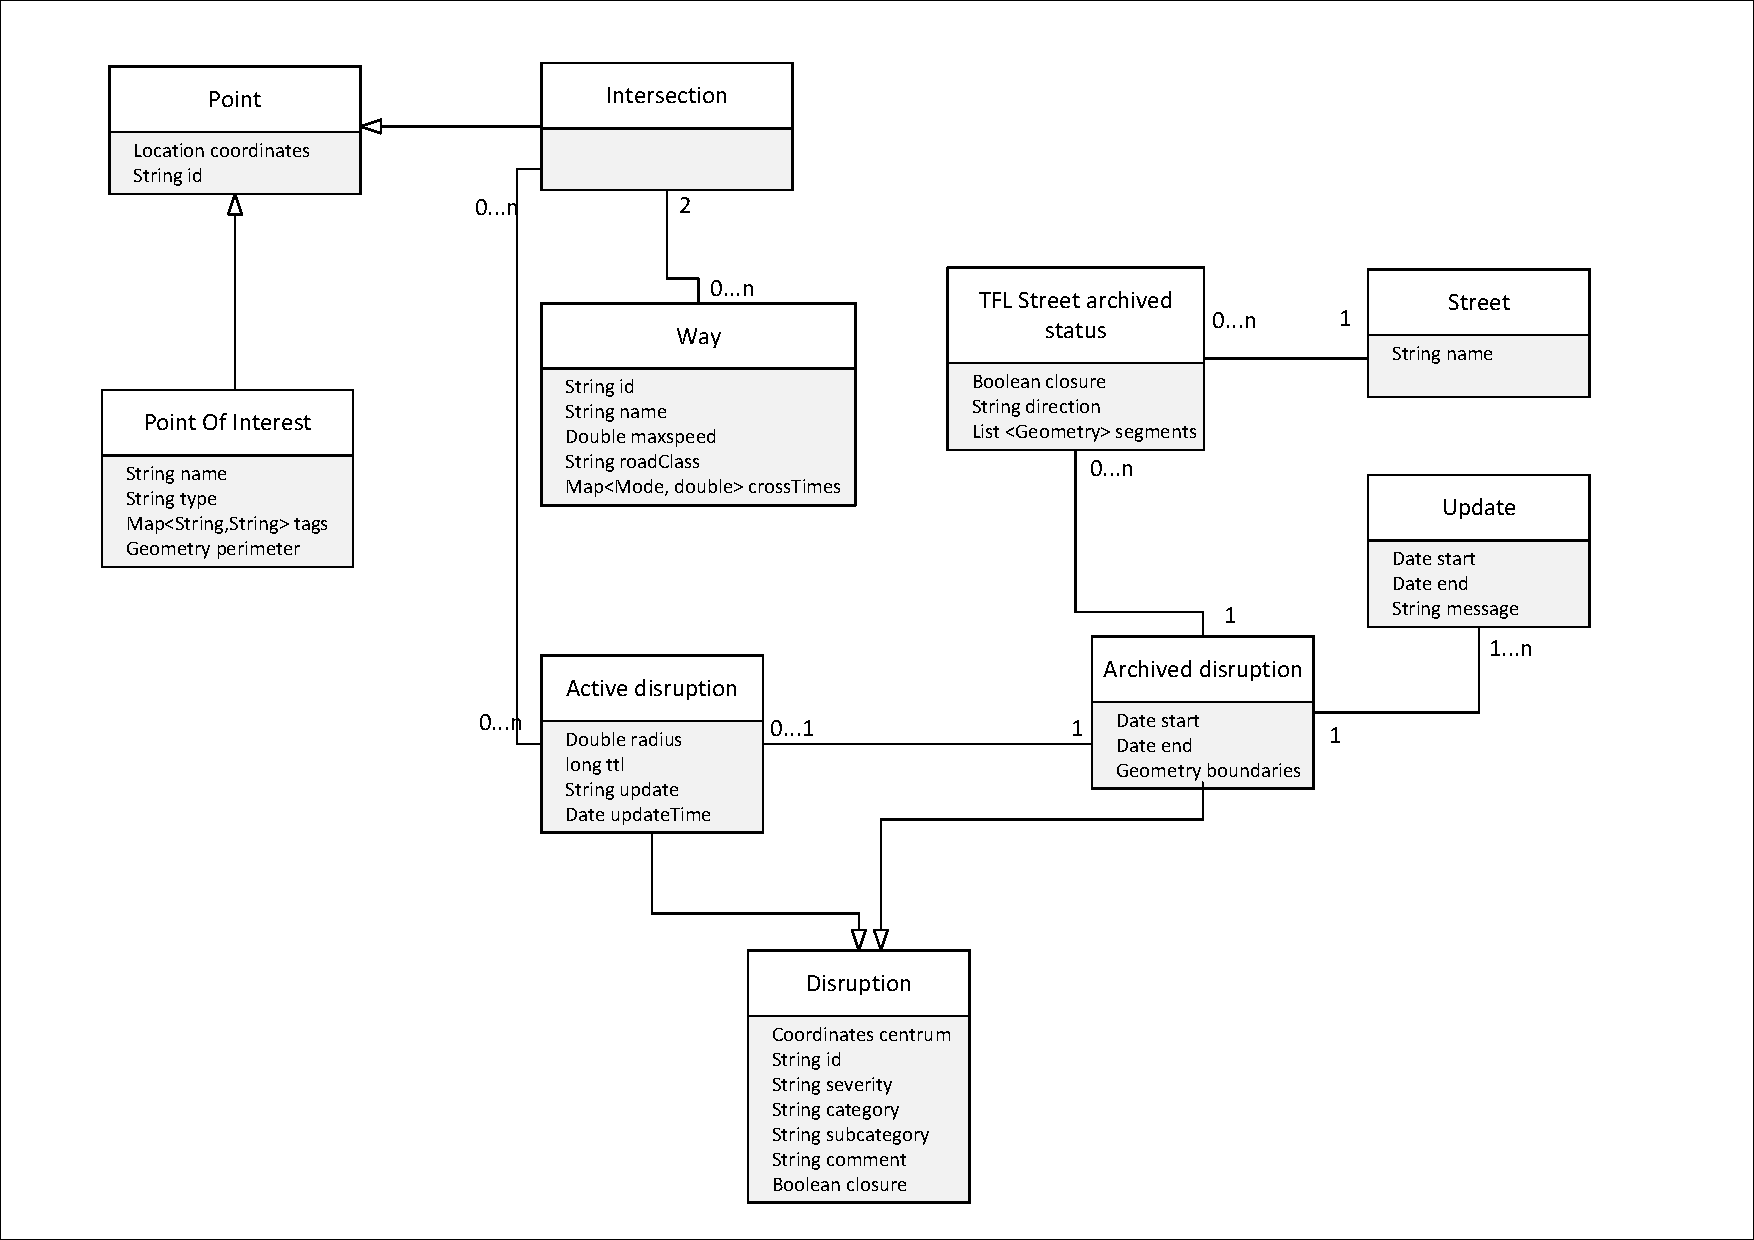
\includepdf[landscape=true,pagecommand=\thispagestyle{plain}]{assets/uml.pdf}

\chapter{Data model}

\paragraph{}
The data model section includes a description of the document collections, 
graph nodes and keys that are stored in the database. Two types of DBMSes have 
been selected for this purpose. 

\paragraph{Document DB}
MongoDB has been chosen as the database management system for the document 
database part, which stores information about the Point Of Interest and the 
concluded disruptions.

The decision to use a document database was based on its flexibility and 
ability to perform complex queries and works as a way to store an history of 
these informations.

\paragraph{Graph DB}
To manage the routing, where users can insert two points and the application will compute a travel route between them, a graph database managed using Neo4j has been selected to better support these features.

\section{Document database}

\paragraph{DBMS} Our choice for the \textit{database management system} to 
handle the document database was \textit{MongoDB}, since it is the most popular 
\textit{DBMS} of its kind and it also provides several functionalities useful 
for our use case, such as indexes and a powerful query engine.

\paragraph{Collections} In MongoDB we created the following collections:

\begin{itemize}
	\item POIs
	\item Disruptions
\end{itemize}

\subsubsection{Point of Interest}
The POIs collection looks like this:

\lstinputlisting{../../schema/example.poi.json}

Where the map \textit{tags} has not a particular structure, but it stores the 
\textit{OpenStreetMap}'s tag for that particular POI. It might store 
information such as its website, its opening hours, its physical dimensions, if 
it is accessible in a wheelchair etc...

\paragraph{Main fields}
\begin{itemize}
	\item \texttt{coordinates} a \textit{GeoJson} document of type 
	\texttt{Point} representing the geographical location of the object
	
	\item \texttt{name} the name of the object, if any
\end{itemize}

\subsubsection{Disruption}
The disruption collection is organized in the following structure:

\lstinputlisting{../../schema/example.disruption.json}

This representation might allow in the future to store additional optional 
values for certain kinds of POIs if the need arises, without any compatibility 
issue for the existing code; for example one might want to store a restaurant’s 
opening hours or the accessibility level for wheelchair users in a certain 
building.

\paragraph{Main fields}
\begin{itemize}
	\item \texttt{boundaries} a \textit{GeoJson} document that could be both of 
	class \texttt{Polygon} or \texttt{Multipolygon}, it represents the effected 
	area. It might not be present in all documents.
	
	\item \texttt{coordinates} the main point effected by the disruption, that 
	is where the application is supposed to draw the sign.
	
	\item \texttt{streets} a list of streets effected by the disruptions and if 
	are closed or not to the traffic
	
	\item \texttt{updates} an archive of updates that \textit{Transport for 
	London} has published
\end{itemize}

\section{Graph database}

\paragraph{DBMS} Our choice for the \textit{database management system} to 
handle the graph database was \textit{Neo4j}, since it can easly handle a huge amount of nodes.


\paragraph{Data} The graph DB is mainly used to store the road network of London and the current active disruption, this is needed so that the routing algorithm can avoid adding to the frontier nodes in an area affected by a closure or increase the weight of nodes in areas affected by critical disruptions.

\paragraph{Schema}For the map side of things we store one class of node and one class of relationship:

\begin{itemize}
	\item \textbf{Intersection }(due to a mistake it is actually called Point 
	in the database) represents the connection between one or more ways, it is 
	a \textit{vertex} of the graph
	
	\lstinputlisting{../../schema/example.point}
	
	\begin{itemize}
		\item \texttt{coord} Those are the geographical coordinates of the 
		node
	\end{itemize}
	
	\item \textbf{Connects} represents the connection between two Insersection. 
	It stores informations like its name and the cost of traversing it and 
	eventual access restrictions, like one way streets or motor-only roads
	
	\lstinputlisting{../../schema/example.connects}
	
	\begin{itemize}
		\item \texttt{maxspeed} It is the maximum speed on that stretch of road 
		expressed in meters per second
		
		\item \texttt{crossTime} It is the estimated crossing time of the edge 
		for each transportation mode. If the cross time is $\infty
		$ then it means 
		that the road has an access restriction in that direction, such has no 
		entry signs.
		
		It was used to use with the \textit{GDS}' implementation of 
		\textit{A*}, since we have implemented our version of \textit{A*} we 
		only check for $\infty$
		
		\item \texttt{class} The road class in the hierarchy where 
		\textit{motorway} is at the top.
	\end{itemize}
	
\end{itemize}

For the disruption handling we have the following nodes and relationships:

\begin{itemize}
	\item \textbf{Disruption} a node in the graph containing all the 
	informations about an active disruption
	
	\lstinputlisting{../../schema/example.disruption}
	
	We save in this edge all the information that could be of immediate help to 
	the user, to avoid making another query to the other databases when 
	requesting a preview of the data. In particular we store:
	
	\begin{itemize}
		\item \texttt{ttl} It is the \textit{Time to live}, that is the number 
		of seconds that remains to programmed end of the disruption, so that if 
		there are problems in the \textit{driver TIMS} the \textit{DBMS} can 
		drop it
	\end{itemize}
	
	\item \textbf{isDisrupted} is a relation between a Point and a Disruption, 
	telling that the road is being affected by a disruption.
	
	We don't store any information on those edges.

\end{itemize}
	
\begin{figure}[H]
	\centering
	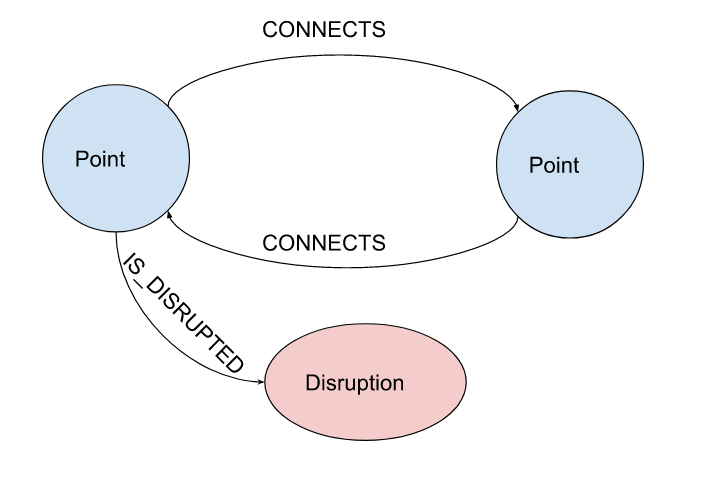
\includegraphics[width=0.7\linewidth]{assets/schemaneo4j}
	\caption{A possible portion of graph}
	\label{fig:schemaneo4j}
\end{figure}






\chapter{Distributed database}
\chapter{Overall platform architecture}

The application has been developed utilizing the Java programming language and the Intellij integrated development environment. As outlined in the Data Model section, MongoDB and Neo4j were chosen as the NoSQL database management systems for data storage and management. It was previously stated that there are three replicas implemented for MongoDB, and a single replica for Neo4j.
\chapter{Framework used}